\documentclass{article}
\usepackage{amsmath}
\usepackage{tikz}
\usetikzlibrary{positioning}

\title{idris-mode: Idris interaction with emacs}
\author{Hannes Mehnert\\\texttt{hannes@mehnert.org}}
\begin{document}
\sloppy
\maketitle

\begin{abstract}
This document describes the interaction of the Idris compiler with the editor emacs, to facilitate a lightweight development environment for Idris programs in emacs.

The goal of the IDE mode is to provide from Idris a structured input and output command processor, which supports all features available in the command line version of the Idris compiler.
\end{abstract}

\section{Introduction}
Getting dependently typed programs right is harder than usual statically typed programs, since the type system is more expressive.
Actually, the type checker of a dependently typed programming language can assist the programmer to develop a type correct program.

In this document we explain the interaction between Idris and emacs, this not a user guide for idris-mode.
The goal is to enable developers to extend idris-mode, as well as use Idris's IDE mode for other editors or tools.

The motivation for IDE mode is to provide an interface for Idris with structured input and output.
The motivation for idris-mode is to have a lightweight development environment for Idris within emacs.

A lot of inspiration for the interaction between Idris and emacs comes from SLIME, the superior LISP interaction mode for emacs~\footnote{not the German punk band ;)}.
The communication protocol is of asynchronous request-reply style: a single request from emacs is handled by Idris at a time.
Idris waits busily for a request on its standard input stream, and outputs the answer to standard output.
The result of a request can be either success or failure, and furthermore, before the result is delivered there might be informal messages.
Since a request can take an arbitrary amount of time, and emacs is single-threaded, the communication happens in an asynchronous fashion: instead of busy waiting for a reply, the requestor gives a continuation which is later called with the result.

\section{Features}
The idris-mode provides basic syntax highlighting for Idris, located in \texttt{idris-syntax.el} (not in scope of this document).
Also indentation is handled in idris-mode, implemented in \texttt{idris-simple-indent.el}.

The currently supported features which interact with the Idris compiler are a read-eval-print-loop (REPL), type checking of Idris files, processing and displaying of errors, a proof mode, case splitting, and other interactive features.

The REPL is useful on its own, and can be started by \textsf{M-x idris-repl}.
This creates a new buffer \emph{*idris-repl*}, whose interaction is very similar to the command-line REPL.
A history, available via C-down and C-up, of previous entered statements is present.
The search in the history uses the currently entered string for its prefix search to find available items.
Automatic completion of available commands is available via tab.

When working on an Idris file, the key C-c C-l loads the file of the current buffer and starts a REPL which has this as its context.
Also, if Idris presented errors while parsing or type checking the file, these are presented in the buffer as orange overlays with tooltips containing the error.

The interactive features: displaying the type of the current name, case splitting, add missing cases, add clause, insert with block, and proof search are all implemented synchronously.
Each feature is bound to a key in the idris-mode keymap.

Inspiration for the proof mode is taken from proof general~\cite{proofgeneral}, an emacs interface for a lot of interactive proof assistants like Coq, Isabelle, PVS.
The proof mode consists of three buffers, one shows the proof obligation, another the proof script, and the third the proof shell.
The proof script buffer highlights the processed parts of the proof script.
There are keybindings available to step forward and backwards over the proof script, namely C-n and C-p.
Additionally, completion of partially written proof script is supported and bound to the key tab.
To get into proof mode, start proving a hole by typing \textsf{:p hole} at the REPL.

Help for the current modes is available, as usual, by C-h m.

\section{Communication}\label{sec:protocol}
The request-reply communication uses the standard input and standard output stream of Idris.
A reply can consist of multiple messages: any number of messages to inform the user about the progress of the request or other informational output, and finally a result, either ``ok'' or ``error''.

The wire format is the length of the messages, encoded in 6 characters hexadecimal, followed by the message encoded as S-expression (sexp).
Additionally, each request includes a unique integer (counting upwards), which is repeated in all messages corresponding to that request.

An example interaction from loading the file \texttt{/home/hannes/empty.idr} looks as follows on the wire:
\begin{verbatim}
00002a((:load-file "/home/hannes/empty.idr") 1)
000039(:write-string "Type checking /home/hannes/empty.idr" 1)
000026(:set-prompt "*/home/hannes/empty" 1)
000032(:return (:ok "loaded /home/hannes/empty.idr") 1)
\end{verbatim}

The first message is the request from idris-mode to load the specific file, which length is hex 2a, decimal 42 (including the newline at the end).
The request identifier is set to 1.
The first message from Idris is to write the string ``Type checking /home/hannes/empty.idr'', another is to set the prompt to ``*/home/hannes/empty''.
The answer, starting with \texttt{:return} is \texttt{ok}, and additional information is that the file was loaded.

There are three atoms in the wire language: numbers, strings, and symbols.
The only compound object is a list, which is surrounded by parenthesis.
The syntax is given in Figure~\ref{fig:syntax}.

\begin{figure}
\centering
\begin{align*}
\mathcal{A}{~::=~}&\mathit{Num} \mid \texttt{"} \mathit{Alpha*} \texttt{"} \mid \texttt{:}\mathit{Alpha*}\\
\mathcal{S}{~::=~}&\mathcal{A} \mid \texttt{(} S \texttt{)} \mid \texttt{nil}
\end{align*}
\caption{Syntax of the wire language, where Num is a positive integer and Alpha is a character, nil is reserved for the empty list}
\label{fig:syntax}
\end{figure}

The state of the Idris process is mainly the active file, which needs to be kept synchronized between the editor and Idris.
This is achieved by the already seen \emph{LoadFile} command.

The full list of supported commands is the data structure \emph{IdeModeCommand} in \texttt{Idris/IdeMode.hs}, and explained in further detail in the following.

\begin{verbatim}
data IdeModeCommand  = REPLCompletions String
                     | Interpret String
                     | TypeOf String
                     | CaseSplit Int String
                     | AddClause Int String
                     | AddProofClause Int String
                     | AddMissing Int String
                     | MakeWithBlock Int String
                     | ProofSearch Int String [String]
                     | LoadFile String
\end{verbatim}

\paragraph{REPLCompletions} returns all possible commands for the given partial string by using the Haskeline completions (\emph{replCompletion} in \texttt{Completion.hs}).

\paragraph{Interpret} interprets the given string as a REPL command.

\paragraph{TypeOf} returns the type of the given top-level name.

\paragraph{CaseSplit} returns the cases for the given name.

\paragraph{AddClause} returns the definition for the given type.

\paragraph{AddProofClause} returns the proof clause for the given name.

\paragraph{AddMissing} returns the missing cases for the given name.

\paragraph{MakeWithBlock} returns a with block for the given name.

\paragraph{ProofSearch} returns a proof for the given name.

\paragraph{LoadFile} loads the given file.

Possible replies include a normal reply:
\begin{verbatim}
:return (:ok SEXP)
:return (:error String)
\end{verbatim}

Informational and abnormal replies
\begin{verbatim}
:write-string String
:set-prompt String
:warning (FilePath, Int, String)
\end{verbatim}

Specially for proof mode
\begin{verbatim}
:start-proof-mode
:write-proof-state [String]
:end-proof-mode
:write-goal String
\end{verbatim}

\section{Implementation}
The implementation of these features are twofold: the emacs side and the Idris side.

\subsection{Idris side}
On the Idris side, the marshaling and unmarshaling of sexps is done in \texttt{IdeMode.hs}.
The main entry point is \emph{idemodeStart}, called by \emph{idrisMain} (both in \texttt{REPL.hs}).
Also, the \emph{idris\_outputmode} field in the \emph{IState} record (in \texttt{AbsSyntaxTree.hs}) is set to \emph{IdeMode 0} (by a call \emph{setIdeMode True} from \emph{idrisMain}).

In the Idris source base, instead of writing raw data to standard output (eg by using \emph{putStrLn}), which violates the protocol presented in Section~\ref{sec:protocol}, Idris uses \emph{ihputStrLn :: Handle $\rightarrow$ String $\rightarrow$ Idris ()}.
This function does a case analysis of the \emph{idris\_outputmode} field in the \emph{IState} record, and either uses \emph{putStrLn} for \emph{RawOutput} (actually \emph{hPutStrLn}) or first converts the message to a sexp by using \emph{convSExp} and wraps it into a \emph{:write-string} message, as seen on line 2 of our example.

To display a result for a command, \emph{ihPrintError} and \emph{ihPrintResult} are available (for failure and success).
Furthermore, the function \emph{ihWarn} produces a warning message, given a source location (\emph{FC} from \texttt{Core/TT.hs}) and a message.

Most of Idris works via IDE mode, for the time being setting the log level greater 5 results in calls to \emph{Debug.Trace.trace} from \texttt{Core}, which uses \emph{unsafePerformIO} and thus is not encapsulated in a sexp.
Also not supported is the execution of programs (\emph{Execute}), to support this the input and output streams of the executed program will need to be wrapped into sexps.

\subsection{Emacs side}
The emacs side is mainly implemented in \texttt{inferior-idris.el}, which provides both an asynchronous (\emph{idris-eval-async}) and a synchronous (busy waiting \emph{idris-eval}) function for interaction.
A dependency diagram of the various emacs lisp files is shown in Figure~\ref{fig:elisp-deps}.

\begin{figure}
\centering
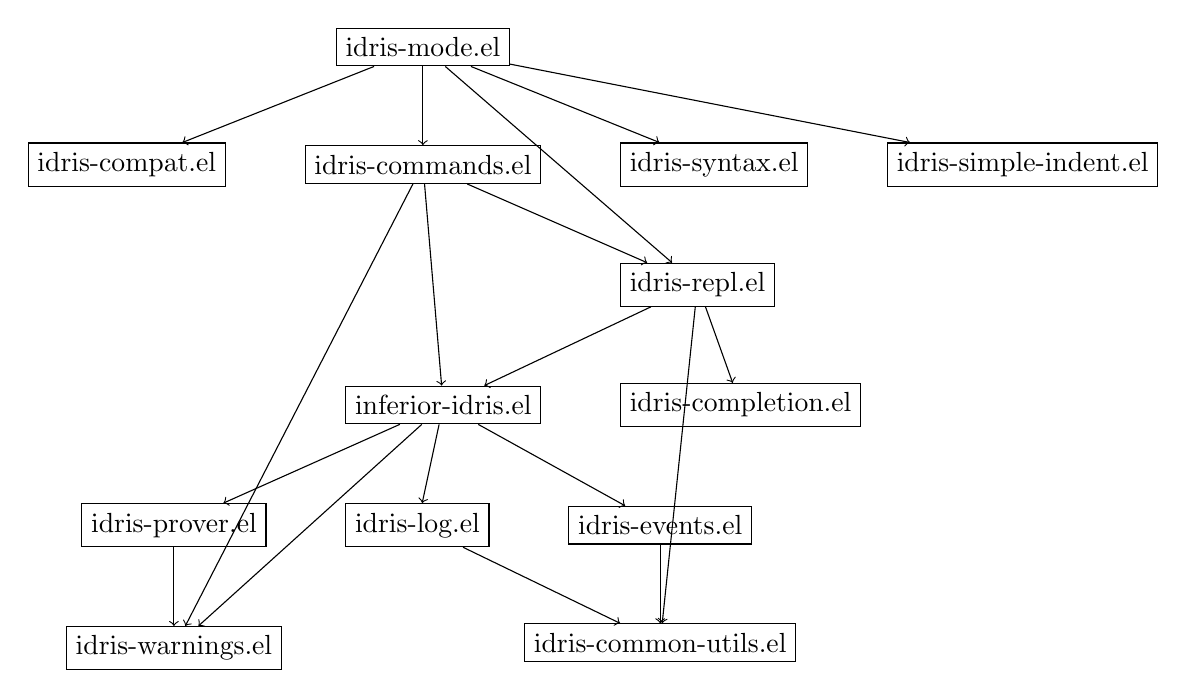
\begin{tikzpicture}
  \tikzstyle{every node}=[draw]
  \node (im) {idris-mode.el};

  \node (commands) [below=of im] {idris-commands.el};

  \node (repl) [below right=of commands] {idris-repl.el};

  \node (inferior) [below left=of repl] {inferior-idris.el};
  \node (completion) [right=of inferior] {idris-completion.el};

  \node (prover) [below left=of inferior] {idris-prover.el};
  \node (log) [right=of prover] {idris-log.el};
  \node (events) [right=of log] {idris-events.el};

  \node (warnings) [below=of prover] {idris-warnings.el};

  \node (common) [below=of events] {idris-common-utils.el};
  \node (compat) [left=of commands] {idris-compat.el};
  \node (syntax) [right=of commands] {idris-syntax.el};
  \node (indentation) [right=of syntax] {idris-simple-indent.el};

  \draw [->] (im) -- (syntax);
  \draw [->] (im) -- (indentation);
  \draw [->] (im) -- (repl);
  \draw [->] (im) -- (commands);
  \draw [->] (im) -- (compat);

  \draw [->] (events) -- (common);
  \draw [->] (log) -- (common);

  \draw [->] (commands) -- (inferior);
  \draw [->] (commands) -- (repl);
  \draw [->] (commands) -- (warnings);

  \draw [->] (repl) -- (common);
  \draw [->] (repl) -- (completion);
  \draw [->] (repl) -- (inferior);

  \draw [->] (inferior) -- (events);
  \draw [->] (inferior) -- (log);
  \draw [->] (inferior) -- (warnings);
  \draw [->] (inferior) -- (prover);

  \draw [->] (prover) -- (warnings);

\end{tikzpicture}
\label{fig:elisp-deps}
\caption{The internal dependency graph of idris-mode}
\end{figure}

Minor notes on some of the implementation files: \texttt{compat.el} includes emacs 24.1 compatibility; \texttt{completion.el} implements a completion popup; \texttt{warnings.el} does the highlighting of warnings using overlays.

The current design uses exactly one idris process for the interaction (a handle is stored in \emph{idris-process} (in \texttt{inferior-idris.el})).

Since it can consume an arbitrary amount of time to handle a request, \emph{idris-eval-async} (in \texttt{inferior-idris.el}) can be used to evaluate any sexp, where the given continuation is called with the asynchronous result.
Some features, like tab completion, return a result immediately.
To simplify understanding of code, idris-mode waits for the reply in a synchronous fashion.
This is achieved by \emph{idris-eval} (as well in \texttt{inferior-idris.el}), which takes a sexp and returns the result immediately.

Both methods of interaction use the same underlying mechanism, namely sending a sexp via \emph{idris-rex} using the dispatcher \emph{idris-dispatch-event}.

The main entry for interaction between emacs and Idris is the method \emph{idris-run} in the \texttt{inferior-idris.el} file.
It starts the idris binary with the \emph{--ide-mode} command line option, and additional customizable flags \emph{idris-interpreter-flags}.
The output of the idris process is connected to \emph{idris-output-filter}, which inserts the received string into the \emph{*idris-process*} buffer.
This buffer is read by \emph{idris-process-available-input}, which validates the string and constructs a sexp (s-expression), which is then logged (to the \emph{*idris-events*} buffer via \emph{idris-event-log} in \texttt{idris-events.el}) and passed to the main dispatcher in \emph{idris-dispatch-event}.

The dispatcher first calls the registered hooks (at the moment, logger, warning and prover, setup by \emph{add-hook 'idris-event-hooks} in \emph{idris-run}; furthermore repl, registered in \texttt{idris-repl.el}, directly in the \emph{idris-repl-mode}) in order until one handled the sexp.
If the sexp is a request (starts with \emph{:emacs-rex}), the given continuation is pushed onto the list of continuations, and the sexp is sent to idris, after being marshalled.
If the sexp is a result (starts with \emph{:result}), the continuation registered during the request is called.
Furthermore, the continuation is removed from the list.

The implementation of the REPL consists of a custom buffer, \emph{*idris-repl*}, which has a prompt (set by the message \emph{:set-prompt}), and several markers: where to put output and results, where to put the prompt and what is the unprocessed user input.
The REPL also has a persistent history, which is saved to \texttt{.idris/idris-history.eld}.
It consumes all \emph{:write-string} messages and inserts the received string to the output; furthermore \emph{:set-prompt} messages are used to update the prompt.

When logging is enabled, log messages are appended to the \emph{*idris-log*} buffer.

The proof mode consists of three buffers and is enabled by the \emph{:proof} command on the REPL.
The Idris prover (\texttt{Prover.hs}) sends the message \emph{:start-proof-mode}, which then opens the buffers \emph{*idris-proof-obligations*}, \emph{*idris-proof-shell*}, and \emph{*idris-proof-script*} in emacs.
Proof obligations are shown in the \emph{*idris-proof-obligations*} buffer, which is readonly.
There are keyboard shortcuts in the \emph{*idris-proof-script*} buffer available to step forward and backward over the proof script.
Furthermore, tab completion is available there as well as in the proof shell.
The proof script highlights the parts which have been processed by Idris.

\section{Highlighting}
Idris mode supports highlighting the output from Idris.
In reality, this highlighting is controlled by the Idris compiler.
Some of the return forms from Idris support an optional extra parameter: a list mapping spans of text to metadata about that text.
Idris mode then uses this list both to highlight the displayed output and to enable richer interaction by having more metadata present.

A particular semantic span is a three element list.
The first element of the list is the index at which the span begins, the second element is the number of characters included in the span, and the third is the semantic data itself.
The semantic data is a list of lists.
The head of each list is a key that denotes what kind of metadata is in the list, and the tail is the metadata itself.
Presently, the following keys are available:
\begin{description}
\item[name] gives a reference to the fully-qualified Idris name
\item[implicit] provides a Boolean value that is True if the region is the name of an implicit argument
\item[decor] describes the category of a token, which can be ``type'', ``function'', ``data'', ``keyword'', or ``bound''.
\item[source-loc] states that the region refers to a source code location. Its body is a collection of key-value pairs, with the following possibilities:
  \begin{description}
  \item[filename] provides the filename
  \item[start] provides the line and column that the source location starts at as a two-element tail
  \item[end]  provides the line and column that the source location ends at as a two-element tail
  \end{description}
\item[text-formatting] provides an attribute of formatted text. This is for use with natural-language text, not code, and is presently emitted only from inline documentation. The potential values are ``bold'', ``italic'', and ``underline''.

\end{description}

The spans emitted by Idris may completely contain another span, but they will never overlap non-hierarchically. That is, one span may be either completely outside the others or contained entirely within another span.
Presently, spans only overlap in output from documentation strings, but this may change in the future.

\section{Conclusion}
The IDE mode provides a structured output of the Idris compiler.
This is especially useful for interfacing Idris to use for interactive development.
It exposes some internals of the Idris compiler which are useful for interactive development environments.

\section{Bugs and Future Work}
The proof mode needs some further thinking, currently it rewrites the proof script with the one from Idris and applies its own indentation (2 whitespaces).
It should be more interactive and not reformat proof script typed in by a user.

The interactive commands also depend heavily on lines and just insert or rewrite the next line.
This should be prevented to avoid brittleness.

As mentioned in the implementation section, not all commands of the Idris REPL are available in IDE mode:
\begin{itemize}
\item Setting the log level greater 5 results in calls to \emph{Debug.Trace.trace}, which uses \emph{unsafePerformIO} and thus is not encapsulated into a sexp.
\item The execution of programs (\emph{Execute}) is not supported, because the input and output streams of the executed program are not wrapped into sexps.
\end{itemize}

\subsection{Future}

Also, navigation in the source code and further support for the developer.
\end{document}
